\documentclass{article}
\usepackage[english]{babel}
\usepackage[utf8]{inputenc}
\usepackage{fancyhdr}
\usepackage[margin=1in]{geometry}
\usepackage{mathtools}
\usepackage{amssymb}
\usepackage{bm}
\usepackage{amsthm}
\usepackage{blindtext}
\usepackage{natbib}
\usepackage{xcolor}
\usepackage{graphicx}
\usepackage{tikz}
\setcounter{subsection}{-1}
\newcommand{\N}{\mathbb{N}}
\newcommand{\R}{\mathbb{R}}
\newcommand{\Q}{\mathbb{Q}}
\newcommand{\x}{\mathbf{x}}
\newcommand{\y}{\mathbf{y}}
\newcommand{\Z}{\mathbb{Z}}
\newcommand{\norm}[1]{\left\lVert#1\right\rVert}
\newcommand{\LL}{\mathcal{L}}
\newcommand{\Prr}[1]{\text{Pr}\left(#1\right)}


\theoremstyle{definition}
\newtheorem{proposition}{Proposition}[section]
\newtheorem{theorem}{Theorem}[section]
\newtheorem{definition}{Definition}[section]
\newtheorem{corollary}{Corollary}[section]
\newtheorem{example}{Example}[section]
\newtheorem{remark}{Remark}[section]
\usepackage{cleveref}
\title{Real Analysis}
\author{Noah Jussila}
\date{\today}

\begin{document}
	\maketitle
	\bibliographystyle{chicago}
	\tableofcontents

\section{Preliminaries}
\subsection{Logic}
\subsection{Sets}
\subsection{Functions}

\section{The Real Numbers}
We begin by returning to the most basic concepts in math. What exactly is a number? We begin with the most basic possible set of numbers, and use those to define more complex sets of numbers, with our goal being to define the real numbers. Lastly, we will look at the ``size'' of these sets, and explore the concept of infinity. 
\subsection{Natural Numbers, Integers, and Rational Numbers}
First, a cursory overview of several sets of numbers is in order. It is given for the sake of exposition, and to illustrate how we define sets of numbers using previously defined sets. For the sake of time, the formal definition of the standard operations (addition, multiplication, etc.) on these sets will be forgone. Rest assured that the operations we are all familiar with are well defined on these sets, and this can be shown rigorously. An excellent reference for this within the context of real analysis can be found in \cite{tao2006analysis}, who takes nothing as given. 

 The most basic numbers are those we use to count. We will call these natural numbers. \begin{definition}
Define the set $ \N\coloneqq\{0,1,2,\ldots\} $ to be the \textit{{\color{red} natural numbers}}. 
\end{definition}
\noindent The operations of addition and multiplication are well defined on $ \N $, in that when adding or multiplying natural numbers, the result is a natural number. A more succinct way of putting this is saying that $ \N $ is \textit{closed} under addition and multiplication. While the natural numbers are great for things such as counting (a fact we will return to), it fails to be useful for much more. In particular, two basic operations we are familiar with are not well defined on $ \N $.
\begin{example}\label{ex1}
	Suppose we want to find the difference in $ 2 $ and $ 5 $, both elements in $ \N $. The difference in question would be $ 2-5 $, but this is not an element of $ \N $! 
\end{example}

In order to address this shortcoming, we need to broaden our view. In effect, we need to ``add more'' numbers to $ \N $. We want to enlarge the set of natural numbers by the amount necessary for subtraction to be well defined. This can be done by taking the set of all differences of natural numbers. For all intents and purposes, this is how we define the integers. 
\begin{definition}
	Define the set $ \Z\coloneqq\{a-b\mid(a,b)\in\N^2\} $ to be the \textit{\color{red}integers}. Two integers are equal, $ a-b=c-d $, if and only if $ a+d=b+c $.\footnote{The added specification of when integers are equal can be avoided by defining $ \Z $ to be a set of equivalence classes. The equivelence relation $ \sim $ would be defined on $ \N $ as $ (a,b)\sim(c,d) $ when $ a+c=b+d $.}  
\end{definition}
\noindent We will take the ordering of $ \Z $, the negation of elements of $ \Z $, and all arithmetic properties of $ \Z $ to be given. There are two things worth noting. The first is that $ \N\subset\Z $. The identity element $ 0\in\N $ gives $ a-0=a $ for each $ a\in\N $, so any natural number can be written as the difference of two natural numbers. Secondly, we defined $ \Z $ only by using $ \N $. This is crucial, as we will define the rationals only by using $ \Z $, and in turn define the real numbers only by using the rationals.

While subtraction is well defined for $ \Z $, the same does not hold for division. 
\begin{example}
 Take the integers $ -3 $ and 6, and suppose we are interested in the ratio of the prior to the latter. Obviously, $$ \frac{-3}{6}=-\frac{1}{2} ,$$ but this is not an element of $ \Z $. 
\end{example}
We can now ``extend'' the integers to accommodate for division, in a similar fashion to when we defined the integers using the natural numbers. 
\begin{definition}
	Define the set $ \Q\coloneqq\{a/b\mid(a,b)\in\Z^2,\ b\neq0\} $ to be the \textit{\color{red}rational numbers}. Two rational numbers are equal, $ a/b=c/d $, if and only if $ ad=bc $.\footnote{Again we could use equivalence classes to define $ \Q $. The equivelence relation $ \sim $ would be defined on $ \N $ as $ (a,b)\sim(c,d) $ when $ ad=bc $.}  
\end{definition}
\subsection{``Holes'' in $ \Q $}
We now begin where the canonical \cite{rudin1964principles} opens. Our goal has been, and continues to be, to define the most comprehensive set of numbers possible. It may help to visualize what we have done so far with a number line. We can illustrate any ``gaps'' or ``holes'' by using red. This can be seen in Figure 1. 
	\begin{figure}[h]
	\centering
	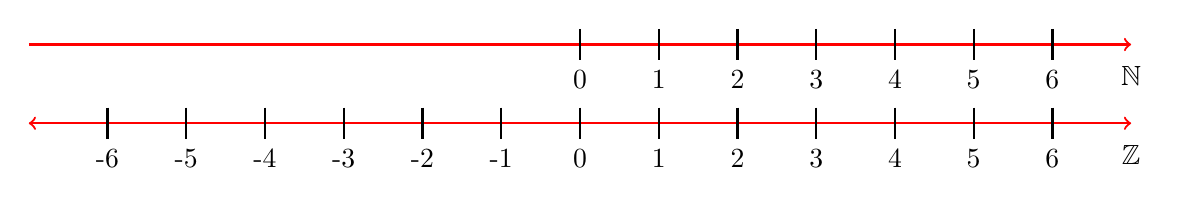
\begin{tikzpicture}
	\draw[thick, red, ->] (0,0) -- (14,0);
	\draw[thick] (7,.2) -- (7,-.2) node[anchor=north] {0};
	\draw[thick] (8,.2) -- (8,-.2) node[anchor=north] {1};
	\draw[thick] (9,.2) -- (9,-.2) node[anchor=north] {2};
	\draw[thick] (10,.2) -- (10,-.2) node[anchor=north] {3};
	\draw[thick] (11,.2) -- (11,-.2) node[anchor=north] {4};
	\draw[thick] (12,.2) -- (12,-.2) node[anchor=north] {5};
	\draw[thick] (13,.2) -- (13,-.2) node[anchor=north] {6};
	\draw (14,-.4) node {$ \N $};
		\draw[thick, red, <->] (0,-1) -- (14,-1);
		\draw[thick] (1,-.8) -- (1,-1.2) node[anchor=north] {-6};
		\draw[thick] (2,-.8) -- (2,-1.2) node[anchor=north] {-5};
		\draw[thick] (3,-.8) -- (3,-1.2) node[anchor=north] {-4};
		\draw[thick] (4,-.8) -- (4,-1.2) node[anchor=north] {-3};
		\draw[thick] (5,-.8) -- (5,-1.2) node[anchor=north] {-2};
		\draw[thick] (6,-.8) -- (6,-1.2) node[anchor=north] {-1};
	\draw[thick] (7,-.8) -- (7,-1.2) node[anchor=north] {0};
	\draw[thick] (8,-.8) -- (8,-1.2) node[anchor=north] {1};
	\draw[thick] (9,-.8) -- (9,-1.2) node[anchor=north] {2};
	\draw[thick] (10,-.8) -- (10,-1.2) node[anchor=north] {3};
	\draw[thick] (11,-.8) -- (11,-1.2) node[anchor=north] {4};
	\draw[thick] (12,-.8) -- (12,-1.2) node[anchor=north] {5};
	\draw[thick] (13,-.8) -- (13,-1.2) node[anchor=north] {6};
	\draw (14,-1.4) node {$ \Z $};
	\end{tikzpicture}
	\caption{The natural numbers and integers ordered number lines.}
\end{figure}
Clearly the natural numbers and integers are not ``comprehensive'' in that they have many gaps. This is what led us to define the rational numbers $ \Q $. It isn't immediate just how well the rationals do at covering the holes in the integers. We can get a sense of this by introducing a property of the rationals. 
\begin{proposition}{(Interspersing of integers by rationals)}\label{prop1}
	For any $ x,y\in\Q $ where $ x<y $, there exists a third rational number $ z\in\Q $ such that $ x<z<y $.
\end{proposition}
\begin{proof}
	Let there be two rationals $ x,y\in\Q $ such that $ x<y $. We can define the third rational number of interest as $ z=(x+y)/2 $. We can show that $ x<z<y $ by using arithmetic.
	\begin{align*}
		x&<y\\\frac{x}{2}&<\frac{y}{2}\\\frac{x}{2}+\frac{y}{2}&<\frac{y}{2}+\frac{y}{2}\\z&<y
	\end{align*} 
	And we can arrive at $ x<z $ by adding $ x/2 $ to each side of the given inequality.
	\begin{align*}
	x&<y\\\frac{x}{2}&<\frac{y}{2}\\\frac{x}{2}+\frac{x}{2}&<\frac{y}{2}+\frac{x}{2}\\x&<z
	\end{align*} 
\end{proof}
\begin{example}\label{ex3}
Take the rational numbers $ 0 $ and $ 1 $. Using the construction given in the previous proof we have $$ \frac{0+1}{2}=\frac{1}{2}$$ is between 0 and 1. We can now repeat this process using the pairs $ (0,1/2) $ and $ (1/2,1) $. \begin{align*}
	\frac{0+1/2}{2}=\frac{1}{4}\\\frac{1/2+1}{2}=\frac{3}{4}
\end{align*}
We could repeat this process an infinite number of times, in effect ``filling in'' gaps in $ \Z $ by successively taking the average of two rational numbers. Figure 2 shows this process on the unit interval in the rationals. 
\begin{figure}[h]
	\centering
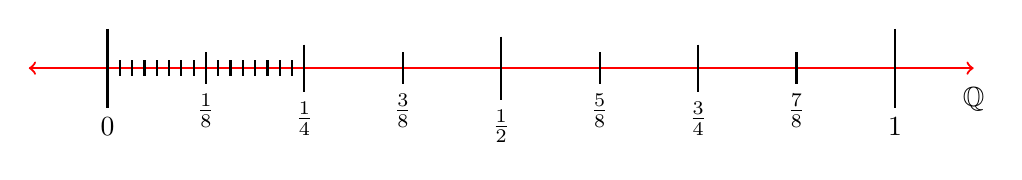
\begin{tikzpicture}
\draw[thick, red, <->] (-1,0) -- (11,0);
\draw[thick] (0,.5) -- (0,-.5) node[anchor=north] {0};
\draw[thick] (5,.4) -- (5,-.4) node[anchor=north] {$ \frac{1}{2} $};
\draw[thick] (2.5,.3) -- (2.5,-.3) node[anchor=north] {$ \frac{1}{4} $};
\draw[thick] (7.5,.3) -- (7.5,-.3) node[anchor=north] {$ \frac{3}{4} $};
\draw[thick] (8.75,.2) -- (8.75,-.2) node[anchor=north] {$ \frac{7}{8} $};
\draw[thick] (1.25,.2) -- (1.25,-.2) node[anchor=north] {$ \frac{1}{8} $};
\draw[thick] (6.25,.2) -- (6.25,-.2) node[anchor=north] {$ \frac{5}{8} $};
\draw[thick] (3.75,.2) -- (3.75,-.2) node[anchor=north] {$ \frac{3}{8} $};
\draw[thick] (10,.5) -- (10,-.5) node[anchor=north] {1};
\draw[thick] (0.15625,.1) -- (0.15625,-.1);
\draw[thick] (0.3125,.1) -- (0.3125,-.1);
\draw[thick] (0.625,.1) -- (0.625,-.1);
\draw[thick] (0.46875,.1) -- (0.46875,-.1);
\draw[thick] (0.78125,.1) -- (0.78125,-.1);
\draw[thick] (0.9375,.1) -- (0.9375,-.1);
\draw[thick] (1.09375,.1) -- (1.09375,-.1);
\draw[thick] (1.40625,.1) -- (1.40625,-.1);
\draw[thick] (1.5625,.1) -- (1.5625,-.1);
\draw[thick] (1.71875,.1) -- (1.71875,-.1);
\draw[thick] (1.875,.1) -- (1.875,-.1);
\draw[thick] (2.03125,.1) -- (2.03125,-.1);
\draw[thick] (2.1875,.1) -- (2.1875,-.1);
\draw[thick] (2.34375,.1) -- (2.34375,-.1);
\draw (11,-.4) node {$ \Q $};

\end{tikzpicture}
\caption{}
\end{figure}\\
The key question is whether or not this fills \textit{all} the gaps in the integers.
\end{example}
While \cref{ex3}, and more formally \cref{prop1}, may lead us to believe that the rational numbers have no gaps, this is unfortunately not the case. There are two classic examples that arise from two of the most basic geometric constructions. 
\begin{example}\label{ex4}
	Suppose we have a circle with diameter $ d $ and circumference $ c $. In this case, the ratio give by $ c/d $ is not an element of the rational numbers. This familiar ratio is written as $ \pi $. For the moment, we can take this as fact. We have not yet developed the tools required to proof that $ \pi\notin\Q $, but we will return to this.  
\end{example}
\begin{example}\label{ex5}
	Suppose there is an isosceles right triangle with legs of length 1, as shown in Figure 3. We want to find the length of the hypotenuse $ x $. 
	\begin{figure}[h]
		\centering
		\begin{tikzpicture}
		\draw[thick] (0,0) -- (8,0);
		\draw[thick] (0,0) -- (0,8);
		\draw[thick] (8,0)--(0,8);
		\draw[thick] (0,0) rectangle (.5,.5);
		\draw[thick] (4,.2)--(4,-.2)node[anchor=north]{1};
		\draw[thick] (.2,4)--(-.2,4)node[anchor=east] {1};
		\draw (4.3,4.3) node {$ x $};
		\end{tikzpicture}
		\caption{}
	\end{figure}\\
This is a simple application of the Pythagorean Theorem. \begin{align*}
	1^2+1^2&=x^2\\2&=x^2
\end{align*}
But this equation has no rational solution, something we can formally prove. 
\end{example}
\begin{proposition}
	There exists no rational number $ x $ which satisfies $ x^2=2 $. 
\end{proposition}
\begin{proof}
	For the sake of contradiction, suppose that there exists a rational $ x $ which satisfies $ x^2=2 $. If this were the case, we could write $ x=m/n $ for some $ m,n\in\Z $, where $ m $ and $ n $ are not both even.\footnote{Otherwise we could write $ x $ in simpler terms as $ m $ and $ n $ would have a common factor of 2.}
\end{proof}
Any $ x $ which does satisfy $ x^2=2 $ would be \textit{irrational}, in that it is not an element of $ \Q $. 
\begin{definition}
	A number is {\color{red}\textit{irrational}} if it is not an element of $ \Q $. 
\end{definition}
\noindent There are \textit{many} irrational numbers, each of which is a gap in the rationals (see Figure 4). 
	\begin{figure}[h]
	\centering
	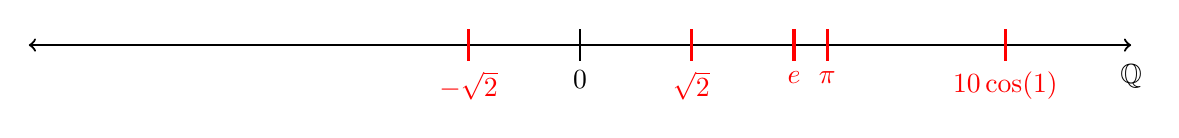
\begin{tikzpicture}
	\draw[thick] (7,.2) -- (7,-.2) node[anchor=north] {0};
	\draw[thick, black, <->] (0,0) -- (14,0);
	\draw (14,-.4) node {$ \Q $};
	\draw[very thick, red ] (10.1415,.2) -- (10.1415,-.2) node[anchor=north] {\color{red}$ \pi $};
	\draw[very thick, red ] (8.4142,.2) -- (8.4142,-.2) node[anchor=north] {\color{red}$ \sqrt{2} $};
	\draw[very thick, red ] (5.5858,.2) -- (5.5858,-.2) node[anchor=north] {\color{red}$ -\sqrt{2} $};
	\draw[very thick, red ] (9.7182,.2) -- (9.7182,-.2) node[anchor=north] {\color{red}$ e $};
		\draw[very thick, red ] (12.403,.2) -- (12.403,-.2) node[anchor=north] {\color{red}$ 10\cos(1) $};
	\end{tikzpicture}
			\caption{}
\end{figure}\\
Our goal now becomes defining a set of numbers that includes not only the rationals, but also all of the irrationals. We began with the natural numbers, and then defined a set $ \Z $ which included the additive inverses of the natural numbers. Then we filled more of the gaps in the integers by taking the ratios of integers. We are now faced with the task of defining a set which eliminates the gaps caused by irrational numbers, and doing so eniterly with the set $ \Q $. 
\subsection{$ \sup $ and $ \inf $}
Before informally constructing the real numbers, it is worth thinking about why $ \Q $ has these ``holes'', and how it relates to a specific property of sets. It goes without saying that, all the sets of numbers we've discussed up until now have some ordering to them. We can make this formal by defining an ordered set.
\begin{definition}
	An \textit{\color{red}ordered set} is some set $ S $ with a binary relation, denoted by $ < $,\footnote{In this case, ``<'' can mean \textit{any} order. It just so happens that we use the same symbol as the familiar ``less than'' order, because it is the canonical example of such a relation.} which satisfies the following properties:
	\begin{enumerate}
		\item If $ x,y\in S $, then exactly one of the statements $$x<y,\ x=y,\ y<x $$ is true.
		\item If $ x,y,z\in S $, and both $ x<y $ and $ y<z $, then $ x<z $. 
	\end{enumerate}
\end{definition}  
The statement $ ``x<y'' $ is read as ``$ x  $ is less than $ y $.''We could also write $ y>x $ instead of $ x<y $. If we were to negative $ y<x $ (``$ y $ is not less than $ x $''), we would arrive at ``y is either greater than $ x $ or equal to $ x $.'' This is denoted as $ y\ge x $. 
\begin{example}
	The set $ \Q $ is a well ordered set if we define $ < $ in the following way for $ x,y\in\Q $:
	$$ x<y\coloneqq y-x \text{ is a postiive rational number}.   $$ Note that we can only relate objects that belong to $ \Q $. This means that we have no way of comparing rational numbers and the solution to the equation $ x^2=2 $.  
\end{example}
We can use the order relation on an ordered set to define bounds on sets.
\begin{definition}
	Suppose $ S $ is an ordered set, and $ E\subseteq S $. If there exists a $ \beta\in S $ such that $ x\le\beta $ for all $ x\in E $, $ E $ is \textit{\color{red}bounded above}, and $ \beta $ is an \textit{\color{red} upper bound} of $ E $. 
\end{definition}
\begin{definition}
	Suppose $ S $ is an ordered set, and $ E\subseteq S $. If there exists a $ \beta\in S $ such that $ x\ge\beta $ for all $ x\in E $, $ E $ is \textit{\color{red}bounded below}, and $ \beta $ is a \textit{\color{red} lower bound} of $ E $. 
\end{definition}
A subtlety in both definitions that is extremely important, is that upper and lower bounds must be elements of the ordered set $ S $. The next example highlights this. 
\begin{example}
 Take $ \Z $ to be an ordered set with the natural order. Pick the subset $ E=\{-2,-1,2\}\subset \Z $. This set has many upper and lower bounds. For upper bounds we have $ 2,3,4,\ldots $. For lower bounds we have $ -2,-3,-4,\ldots
  $. It may be tempting to say that a fraction such as $ 5/2 $ is an upper bound of $ E $, but it is not. This follows from the fact that $ 5/2\notin \Z $, so we have no means of relating it to elements in $ \Z $. In this particular case, there are upper and lower bounds of the set are included in the set. This need not be the case, as the next example shows.  
\end{example}
\begin{example}
	Let's look at the ordered set $ \Q $, and subset $ E=\{x\in\Q\mid 0<x<1\}\subset \Q $.\footnote{The use of the familiar interval notation of $ (0,1) $ will be properly defined and restricted to the real numbers in the following section.} In this case, each element of $ \{x\in\Q\mid x\le 0\} $ is a lower bound of $ E $, and  each element of $ \{x\in\Q\mid x\ge 1\} $ is an upper bound of $ E $. Even though $ 0,1\notin E $, they are still least and upper bounds of $ E $ respectively. 
\end{example}
\begin{remark}
	It is often obvious what exact order we are talking about when referring to an ordered set, like in the case of $ \Q $ and $ \Z $. In these cases, we'll just assume we're using the natural order.  
\end{remark}
We now will introduce two definitions that correspond to a special type of upper and lower bound.
\begin{definition}
	Suppose $ S $ is an ordered set, $ E\subset S $, and $ E $ is bounded above. We say that $ \alpha $ is a \textit{\color{red}leas- upper-bound} of $ E $ if:
	\begin{enumerate}
		\item $ \alpha $ is an upper bound of $ E $.
		\item If $ \gamma<\alpha $, then $ \gamma $ is not an upper bound of $ E $.
	\end{enumerate}
Alternatively, we can refer to $ \alpha $ as the \textit{\color{red}supremum} of $ E $, and write $ \alpha=\sup E $
\end{definition}
\begin{definition}
	Suppose $ S $ is an ordered set, $ E\subset S $, and $ E $ is bounded below. We say that $ \alpha $ is a \textit{\color{red}greatest-lower -bound} of $ E $ if:
	\begin{enumerate}
		\item $ \alpha $ is a lower bound of $ E $.
		\item If $ \gamma>\alpha $, then $ \gamma $ is not a lower bound of $ E $.
	\end{enumerate}
	Alternatively, we can refer to $ \alpha $ as the \textit{\color{red}infimum} of $ E $, and write $ \alpha=\inf E $
\end{definition}
\begin{remark}
	Both definitions use the definite article \textit{the} before supremum and infimum. This is because they are unique. This is also implied by the use of the superlative \textit{least} and \textit{greatest}. Nevertheless, this is a result of the definition, and can be properly proven. 
\end{remark}

\begin{example}
	If we return to Example 2.7, where $ E=\{-2,-1,2\}\subset\Z $, we have $ \sup E=2 $ and $ \inf E=-2 $. 
\end{example}
\begin{example}
	In example 2.8, $ \inf E=0 $ and $ \sup E=1 $.
\end{example}
\begin{example}
	Sticking with the set $ \Q$, consider the subset $ E=\{x\in\Q\mid x^2\le 2\}\subset \Q $. This set has no supremum, because the number satisfying $ x^2=2 $ is not an element of $ \Q $ (as shown in Proposition 2.2). We will formally prove this fact shortly. 
\end{example}
It is no coincidence that a subset of $ \Q $ fails to have a supremum, because of one of the ``holes'' in $ \Q $. The following definition will help us formalize this relationship. 
\begin{definition}
	Let $ S $ be an ordered set. If for all $ E\subset S $, where $ E $ is nonempty and bounded from above, $ \sup E $ exists, then $ S $ has the \textit{\color{red}least-upper-bound} property. 
\end{definition}
The least-upper-bound property ensures that any nontrivial subset of an ordered set has a supremum in that ordered set. We could define an equivelent property known as the greatest-lower-bound property. The next two propositions serves as nice examples of the least-upper-bound property, or lack there of,  in action.
\begin{proposition}
	The set $ \Z $ has the least-upper-bound property.
\end{proposition}
The idea behind the following proof takes advantage of the fact that $ \Z $ is discrete. For some set $ E\subset \Z $, we can always just look at an upper bound of it, and keep subtracting $ 1 $ until the resulting number is in $ E $. Then we will have found our upper bound.
\begin{proof}
	We will show that an arbitrary nontrivial set $ E\subset \Z $ has a supremum. Let $ x\in E $, and $ \beta $ be an upper bound of $ E $. We know that $ \beta\ge x $ for all $ x\in E $ We can show that $ \sup E $ exists via induction on $ \beta-x $ for our arbitrary $ x\in E $. Our base case is when $ \beta-x=0 $. If this holds, then $ \beta\in E $, so $ \beta\in\Z $ and $ \sup E=\beta $. Now suppose that this statement holds when $ \beta-x=k $ for $ k\in\N $ (this is our induction hypothesis). It is either the case that $ \beta\in E $ or $ \beta\notin E $. If $ \beta\in E $, then $ \sup E=\beta $. If $ \beta \notin E $, then let $ \beta'=\beta -1 $. Then $ \beta' $ is an upper bound of $ E $, and $$\beta'-x=\beta-1-x=\beta-x-1=k+1=1=k .$$ By the induction hypothesis, $ \sup E $ exists.   
\end{proof}
\begin{proposition}
	The set $ \Q $ does not have the least-upper-bound property.
\end{proposition}
To prove this, we will first establish that $ 2 $ is an upper bound of the set defined in Example 2.11, and then show the set has no supremum via contradiction.
\begin{proof}
	If suffices to find a single subset of $ \Q $ which fails to have a supremum. Let that set be $ E=\{x\in\Q\mid x^2\le 2\} $. 
	\begin{enumerate}
		\item Suppose for contradiction that $ 2 $ is not an upper-bound of $ E $. Then there exists an $ x\in E $ such that $ x>2 $. This would imply that $ x^2>4 $, which contradicts the assumption that $ x \in E $. 
		\item Suppose for contradiction that $ E $ has a supremum, and that $ \sup E=\alpha $ for $ \alpha\in\Q $. Define a new rational number $ y\in \Q $ as 
		\begin{equation}\label{key}
		y=\alpha-\frac{\alpha^2-2}{x+2}=\frac{2(\alpha+1)}{\alpha+2}.
		\end{equation}
		Squaring this and subtracting $ 2 $ gives 
		\begin{equation}\label{key}
		y^2-2=\frac{4(\alpha+1)^2}{(\alpha+2)^2}-\frac{2(\alpha+2)^2}{(\alpha+2)^2}=\frac{2(\alpha^2-2)}{(\alpha+2)^2}.
		\end{equation} We can use $ y $ to reach a contradiction in each possible case, those being: $ \alpha^2<2 $, $ \alpha^2=2 $, $ \alpha^2>2 $.
		\begin{enumerate}
			\item Suppose that $ \alpha^2<2 $. This means that $ \alpha^2-2<0 $, so Equation (1) implies that $ y>\alpha $. At the same time, Equation (2) implies that $ y^2-2<0 $, which means $ y^2<2 $. This gives that $ y\in E $, despite the fact that $ \alpha<y $. This contradicts the fact that $ \alpha $ is an upper-bound of $ E $
			\item Suppose $ \alpha^2=2 $. We already know this cannot be the case by Proposition 2.2. 
			\item  Finally, assume that $ \alpha^2>2 $, giving $ \alpha^2-2=0 $. Equation (1)	implies $ y<\alpha $ while Equation (2) implies $ y^2-2>0 $, meaning $ y^2>2 $. This establishes $ y $ as an upper bound for $ E $, but $ y<\alpha $, which contradicts $ \sup E=\alpha $.  
	 	\end{enumerate}
	\end{enumerate}
\end{proof}
The ``holes'' in $ \Q $ are a result of $ \Q $ not having the least-upper-bound property. In order to perform calculus, we need a set that has this property, otherwise things like continuity and differentiation would not work. This property is not sufficient in and of itself though. If that were the case then we would have stopped extending out set of numbers at $ \Z $. We want a set of numbers as ``comprehensive'' as $ \Q $, but with the least-upper-bound property. It turns out, that this (and a whole lot more) is what we will get from the real numbers.  
\subsection{The Real Numbers}
We will now construct the real numbers using only $ \Q $. First, we will define the algebraic structure that the real numbers will take on.
\begin{definition}
	A \textit{\color{red}field} is a set $ F $ with two operations, addition and multiplication, which satisfy the following axioms for all $ x,y,z\in F $:
	\begin{enumerate}
		\item Axioms for addition:
		\begin{enumerate}
			\item $ x+y\in F $ (closed under addition)
			\item $ x+y=y+x $ (commutative)
			\item $ (x+y)+z=x+(y+z) $ (associative)
			\item There exists an element $ 0\in F $ such that $ 0+x=x $ (identity element)
			\item There exists an element $ -x\in F $ such that $ x+(-x)=0 $ (inverse element)
		\end{enumerate}
		\item Axioms for multiplication:
		\begin{enumerate}
			\item $ xy\in F $ (closed under multiplication)
			\item $ xy=yx $ (commutative)
			\item $ (xy)z=x(yz) $ (associative)
			\item There exists an element $ 1\in F $ such that $ 1x=x $ (identity element)
			\item If $ x\neq 0 $, there exists an element $ 1/x\in F $ such that $ x(1/x)=1 $ (inverse element)
		\end{enumerate}
		\item The distributive property:
		$$ x(y+z)=xy+xz$$
	\end{enumerate}
\end{definition}
The study of fields is its own entire subject in math, and lives within the discipline if abstract algebra. For more details about fields, see \cite{dummit2004abstract}. These axioms can be used to reach several familiar conclusions about arithmetic in fields, and can be found as formal propositions in \cite{rudin}. A more specific type of field is that which is also an ordered set.
\begin{definition}
	An \textit{\color{red} ordered field} is a field $ F $ such that
	 \begin{enumerate}
		\item $ x+y<x+z $ if $ x,y,z\in F $ and $ y<z $,
		\item $ xy>0 $ if $ x,y\in F $, $ x>0 $, and $ y>0 $. 
	\end{enumerate}
\end{definition}
\begin{example}
	The set $ \Q $ is an ordered field. 
\end{example}

Our goal is now to construct an ordered field which not only contains $ \Q $, but also has the least-upper-bound property. In order to do this we'll use the fact that $ \Q $ has ``holes'' in it. We'll form a pair of set $ (A,B) $ that partition $ \Q $ such that each of these partitions corresponds to a real number. 

\begin{definition}
	A \textit{\color{red}Dedekind cut} $ x=(A,B) $ is a pair of subsets $ A,B\subset \Q $ satisfying the following:
	\begin{enumerate}
		\item $ A\cup B=\Q $, $ A\cap B=\emptyset $, $ A\neq\emptyset $, and $ B\neq\emptyset $.
		\item If $ a\in A $ and $ b\in B $, then $ a<b $.
		\item $ A $ contains no largest element.
	\end{enumerate}
\end{definition} 
\begin{example}
	Let $ A=\{y\in \Q \mid y<0\} $ and $ B=\{y\in\Q\mid y\ge 0\} $. Our cut is $ x=(A,B) $, and can be seen in Figure 5.
		\begin{figure}[h]
		\centering
		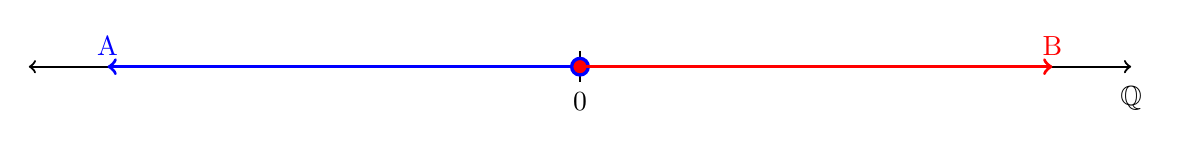
\begin{tikzpicture}
		\draw[thick] (7,.2) -- (7,-.2) node[anchor=north] {0};
		\draw[thick, black, <->] (0,0) -- (14,0);
		\draw (14,-.4) node {$ \Q $};
		\draw[ very thick, blue, ->] (7,0) -- (1,0) node[anchor=south] {A};
		\filldraw[color=blue, fill=red, very thick] (7,0) circle (3pt);
		\draw[ very thick, red, ->] (7,0) -- (13,0) node[anchor=south] {B};
		
		\end{tikzpicture}
		\caption{Dedekind cut corresponding to $ 0\in\Q $.}
	\end{figure}
This cut uniquely represents $ 0\in\Q $, as no other cut can be defined in this way ``at'' $ 0 $. 
\end{example}
\begin{example}
	Perhaps a better example is the cut defined by $ A=\{q\in\Q\mid q\le 0\text{ or }q^2<2 \} $ and $ A=\{q\in\Q\mid q> 0\text{ or }q^2>2 \} $. This cut corresponds to the solution of the equation $ x^2=2 $.  
\end{example}
\begin{definition}
	A \textit{\color{red}real number} is a Dedekind cut in $ \Q $. The set of real numbers is denoted by $ \R $. 
\end{definition}
\begin{definition}
	A real number $ x=(A,B) $ is a \textit{\color{red}rational number} if $ B $ contains a smallest element (namely $ x $).
\end{definition}
\begin{definition}
	A real number $ x=(A,B) $ is a \textit{\color{red}irrational number} if $ B $ contains no smallest element.
\end{definition}
\begin{example}
	The cut defined by $ A=\{y\in \Q \mid y<0\} $ and $ B=\{y\in\Q\mid y\ge 0\} $ is rational, as $ B $ has a smallest element in the form of $ 0 $.  
\end{example}
\begin{example}
	The cut defined by $A=\{q\in\Q\mid q\le 0\text{ or }q^2<2 \} $ and $ A=\{q\in\Q\mid q> 0\text{ or }q^2>2 \} $ has no smallest element. Therefore it is an irrational number. We will denote this particular number as $ \sqrt{2} $. 
\end{example}
Now that we have properly defined $ \R $, we can \textit{finally} refer to the quantity $ \sqrt{2} $! It is no longer a mysterious solution to an equation, and is well defined in $ \R $. This is a relatively small payoff, but the real rewards are the two following theorems. These are the main results of this section, and are of the utmost importance. The first will allow us to perform operations on $ \R $, and the second will play a key role in proving familiar theorems from calculus. The proof of the first result is rather long, and not very informative, so it is omitted. It is important to understand \textit{how} it would be proved though. Before the big reveal, we will define an order on $ \R $
\begin{definition}
	Given real numbers $ x=(A,B) $ and $ y=(C,D) $, we define the following order:$$x\le y\coloneqq A\subseteq C .$$ The inequality is strict if $ A\subset C $. 
\end{definition}
\begin{example}
	Let $ x=2=(A,B)=(\{y\in \Q \mid y<2\},\{y\in\Q\mid y\ge 2\})$, and $ y=3=(C,D)=(\{z\in \Q \mid z<3\},\{z\in\Q\mid z\ge 3\})$. It should come as no surprise that $ 2<3 $, but this is because $ A\subset C $.  
\end{example}
\begin{theorem}
	The set $ \R $ is an ordered field containing $ \Q $.
\end{theorem}
\begin{proof}
	See the appendix of chapter 1 in \cite{rudin}. The idea is that addition and multiplication of cuts must be define, and the all the axioms of fields and ordered fields must be verified using the cut definition of a real number. 
\end{proof}
\begin{theorem}[Completeness of the real numbers]
	The set $ \R $ has the least-upper-bound property.
	\begin{proof}
	We will show an arbitrary nonempty subset of $ \R $ has a supremum. Let $ E\subset \R $, where $ A\neq\emptyset $, have the upper bound $ \beta\in\R $. We may write $ \beta $ as a Dedekind cut, $ \beta=(A,B) $. Additionally, we may express each $ \alpha\in E $ as a cut $ \alpha=(L_\alpha,U_\beta) $. Now we will construct a real number by taking the union of all $ L_\alpha $.
	$$ \gamma=\left(\bigcup_{\alpha\in E}L_\alpha,\Q\backslash \bigcup_{\alpha\in E}L_\alpha\right)=(L,\Q\backslash
	 L)=(L,U)$$  
	I claim that $ \sup E=\gamma $.
	
	First we must verify that $ \gamma\in\R $ by showing that $ (L,U) $ is a valid Dedekind cut, and satisfies the requirements of Definition 2.13: 
	\begin{enumerate}
		\item The set $ E $ is nonempty, so there exists at least one $ \alpha=(L_\alpha,U_\alpha)\in E $. Because $ L_\alpha\neq\emptyset $ and $ U_\alpha\neq\emptyset $ by definition 2.13, we have $ L\neq\emptyset $ and $ U\neq\emptyset $. By the definition of $ U $ as $ \Q\backslash L $, we have that $  L\cup U=\Q$ and $ L\cap U=\emptyset $. 
 		\item {\color{red}FINISH THIS} 
		\item  {\color{red}FINISH THIS} 
	\end{enumerate}
	\end{proof}
Therefore $ \gamma\in\R $. By construction, $ \alpha\le\gamma $ for all $ \alpha\in E $, making $ \gamma $ an upper bound. To show that it is the least-upper-bound, we will now show any number lesser than it cannot be an upper bound. Now suppose $ \delta <\gamma $. This means $  C\subset L $, where $ \delta $ is expressed as a cut $ \delta=(C,D) $. This means there exists some $ s\in L $ such that $ s\notin C $. But $ s\in L $, so it is in $ L_\alpha $ for some $ \alpha\in E $. Hence, $ C\subset L_\alpha $, giving $ \delta <\alpha $. This shows that $ \delta $ is not an upper bound, meaning $ \sup E =\gamma$.
\end{theorem}
\begin{example}
	Consider the set of real numbers $ E=\{-1,-1/2,-1/3,-1/4,\ldots\} $. What is the supremum of this set? Intuitively, it should be $ 0 $, but we can verify this by constructing it like we did in the previous proof. Each number in $ E $ corresponds to a cut $ (L_n,U_n) $, for $ L_n=\{x\in\Q\mid x<-1/n\} $ and $ U_n=\{x\in\Q\mid x\ge -1/n\} $, where $ n\in\N $. Our supremum is $$\gamma=\left(\bigcup_{n\in \N}\{x\in\Q\mid x<-1/n\},\Q\backslash \bigcup_{n\in \N}\{x\in\Q\mid x<-1/n\}\right)=(\{x\in\Q\mid x<0\},\{x\in\Q\mid x\ge0\}). $$ Therefore, $ \gamma=0 $.  
\end{example}
You will often here the real numbers referred to as ``complete'' because they have the least-upper-bound property. This is because the least-upper-bound property ensures there are no `gaps'' in the real line like there are in $ \Q $. Down the road we will introduce a more formal definition of complete.

Finally, we will adopt the familiar notation of intervals in $ \R $, and add make an important addition to $ \R $. 
\begin{definition}
	We will use the following notation to refer to \textit{\color{red} intervals} of $ \R $:
	\begin{align*}
		(a,b)=\{x\in\R\mid a<x<b\}\\
		[a,b)=\{x\in\R\mid a\le x<b\}\\
		(a,b]=\{x\in\R\mid a<x\le b\}\\
		[a,b]=\{x\in\R\mid a\le x\le b\}
	\end{align*}
\end{definition}
\begin{definition}
	The \textit{\color{red}extended real number system} consists of the real field $ \R $ and two symbols: $ \infty $, and $ -\infty $. The original order of $ \R $ is preserved, and we define $$ -\infty <x<\infty$$ for all $ x\in\R $. 
\end{definition}
The extended real numbers do not form a proper field, but we can adopt some conventions for arithmetic using $ \infty $ and $ -\infty $ for $ x\in\R $:
\begin{enumerate}
	\item $ x+\infty=\infty $, $ x-\infty=-\infty $, $ x/\infty=x/-\infty=0 $. 
	\item For $ x>0 $, $ x(\infty)=\infty $, and $ x(-\infty)=-\infty $.
	\item For $ x<0 $, $ x(\infty)=-\infty $, and $ x(-\infty)=\infty $.
\end{enumerate}
\subsection{Properties of $ \R $}
The importance of Theorem 2.2 can not be understated. It is perhaps \textit{the} defining property of $ \R $, and it gives rise to numerous results in analysis. For now, we can use it to prove two additional properties of $ \R $.
\begin{theorem}[Archimedean property of $ \R $]
For $ x,y\in \R $ where $ x>0 $, there exists an $ n\in\N $ such that $ nx>y $.
\end{theorem}   
\begin{proof}
Let $ A $ be the set of all $ nx $ for $ x\in\R $ and $ n\in\N $, where $ x>0 $. For contradiction, suppose that there exists no such $ n\in\N $ such that $ nx>y $ for $ y\in\R $. This makes $ y $ an upper bound of $ A $. By the completeness of $ \R $, $ \sup A=\alpha $ exists. Since $ x>0 $, $ \alpha-x<\alpha $, and $ a-x $ is not an upper bound of $ A $. This means there exists an $ m\in\N $ such that $ a-x<mx $. But this would imply $ \alpha<mx+x=m(x+1) $, where $ (m+1)x\in A $. This contradicts the fact that $ \alpha $ is an upper bound of $ A $. 
\end{proof}
\begin{example}
	Suppose $ x=10 $ and $ y=213 $. By the Archimedean property of $ \R $, we know there exists a multiple of $ 10 $ that is greater than $ 213 $. $$ 10(22)=220>213$$  
\end{example}
\begin{theorem}[$ \Q $ is dense in $ \R $]
For $ x,y\in \R $ where $ x<y $, there exists a $ p\in\Q $ such that $ x<p<y $. 
\end{theorem}  
\begin{proof}
We have $ x<y $, giving $ y-x>0 $. By the Archimedean property (Theorem 2.3), there exists an $ n\in\N $ such that 
\begin{equation}\label{key}
n(y-x)>1.
\end{equation}
We can use Theorem 2.3 to find $ m_1,m_2\in\N $ for which:
\begin{align*}
	m_1>nx,\\m_2>-nx.
\end{align*}
We can combine these two inequalities to conclude $ -m_2<nx<m_1 $. This implies there exists an $ m\in\N $ (with $ -m_2\le m\le m_1 $) such that \begin{equation}\label{key}
m-1\le nx<m.
\end{equation}  
If we combine $ (3) $ and $ (4) $ we get $$ nx<m\le 1+nx<ny.$$ Dividing by $ n $ (which is positive) gives $ x<\frac{m}{n}<y$. 
\end{proof}
The density of $ \Q $ in $ \R $ is both surprising and useful for constructing examples. In practice, it means that every irrational number has a rational number arbitrarily close to it. We can approximate any number in $ \R $ arbitrarily well with a rational number.
\begin{example}
We will now mimic the proof of Theorem 2.4 with actual numbers. We will find a rational $ p\in\Q $ such that $ e<p<\pi $.\footnote{You shouldn't even need to perform the construction to arrive at an answer, as $ e $ and $ \pi $ are not particularly ``close'' to each other. We could for instance take $ p=3 $. } We have $ \pi-e>0 $. We know $$ 3(\pi-e)>1 .$$ Next we pick whole numbers $ m_1=9 $ and $ m_2=8 $, and get the inequality $ 8<3e<9 $. Now take $ m $ to be $ 9 $ and reach our final inequality of $$ 3e<9<1+3e <3\pi.$$ Dividing by $ n=3 $ gives our desired rational number is $ 9/3=3 $.  
\end{example}
\begin{example}
	Let $ \sqrt{2}\in\R $, and let $ \varepsilon>0 $.\footnote{This is the first time we're using the infamous $ \varepsilon $. It just stands in for any arbitrarily small positive number.} By the density of $ \Q $ in $ \R $, there exists $ p\in\Q $ such that $ \sqrt{2}-\varepsilon<p<\sqrt{2} $. This will hold \textit{for all} $ \varepsilon>0 $ so as we let $ \varepsilon $ become smaller and smaller, we will have an increasingly accurate rational approximation of $ \sqrt{2} $.
\end{example}     
\subsection{Cardinality}
So far, I've been intentional in avoiding any discussion of the size of the sets we have been working with. When constructing $ \Z $ from $ \N $, it was never stated that $ \Z $ was somehow ``bigger'' than $ \N $. All we know is that $ \Z $ has elements that $ \N $ does not. The same can be said for $ \Z $ and $ \Q $, or $ \Q $ and $ \R $. It is now time that we turn our attention to this matter, and more generally the size, or ``cardinality'' of sets. 

Determining the size of a set amounts to counting the number of elements in that set. But how do we make the notion of counting formal? We will do this with functions. Before formally defining anything, consider how you may count something. If you are tasked with counting the number of elements in the set $ X=\{a,b,c\} $, you're answer will surely by 3. How did you get that number? You said assigned the number $ 1 $ to $ a $, $ 2 $ to $ b $, and $ 3 $ to $ c $. We should note three different things about this process:
\begin{enumerate}
	\item Each number we use is from $ \N $.
	\item Each element of $ X $ is assigned a number. We wouldn't have counted properly if we skipped some element. 
	\item No number in $ \N $ is assigned to multiple elements in $ X $. We do not want to count multiple elements as a single element.
\end{enumerate}
This process of assigning elements in $ \N $ to those in $ X $ is shockingly similar to the notion of a function, as we are mapping elements from one set to those in another set. Furthermore, the properties we must obey while counting have their own analogous forms with functions: surjectivity, and injectivity. For this reason, we will use functions to formalize the size of a set.

First, we will address the abstract case of when two sets have the same number of elements, and then we will transition to the size of sets.
\begin{definition}
	The \textit{\color{red}cardinality} of a set $ X $, denoted $ |X| $, is the number of elements that belong to the set.   
\end{definition} 
\begin{definition}
	Two sets $ X $ and $ Y $ have \textit{\color{red}the same cardinal number} if there exists a bijection $ f:X\to Y $ from $ X $ to $ Y $.  
\end{definition}  
\begin{example}
	Let $ X=\{1,2,3\} $ and $ Y=\{\sqrt{2},e,\pi\} $. We can define $ f:X\to Y $ as $$ f(x)=\begin{cases}
	\sqrt{2}\text{ if }x=1\\e\text{ if }x=2\\\pi\text{ if }x=3
	\end{cases}.$$
	\begin{figure}[h!]
		\centering
		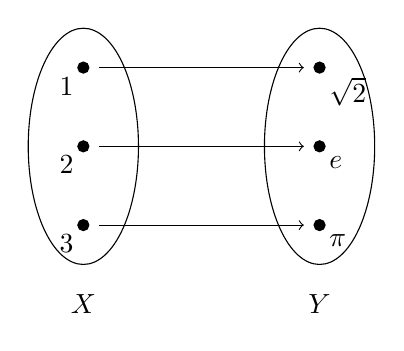
\begin{tikzpicture}
		\draw (0,0) ellipse (0.7cm and 1.5cm);
		\draw (3,0) ellipse (0.7cm and 1.5cm);
			\filldraw (0,0) circle (2pt) node[anchor=north east] {$ 2 $};
			\filldraw (0,1) circle (2pt) node[anchor=north east] {$ 1 $};
			\filldraw (0,-1) circle (2pt) node[anchor=north east] {$ 3 $};
			\filldraw (3,0) circle (2pt) node[anchor=north west] {$ e $};
			\filldraw (3,1) circle (2pt) node[anchor=north west] {$ \sqrt{2} $};
			\filldraw (3,-1) circle (2pt) node[anchor=north west] {$ \pi $};
		
			\draw (0,-2) node {$ X $};
			\draw (3,-2) node {$ Y $};
			\draw[->] (0.2,0) -- (2.8,0) ;
			\draw[->] (0.2,1) -- (2.8,1) ;
			\draw[->] (0.2,-1) -- (2.8,-1) ;
		\end{tikzpicture}
		\caption{Bijection $ f:X\to Y $.}
	\end{figure}  \\
This function is clearly a bijection, and we have that $ |X|=|Y| $.
\end{example} 
\begin{example}
	Let $ \Z^-=\{x\in\Z\mid x<0\} $ and $ \Z^+=\{x\in\Z\mid x>0\} $. There exists a very natural bijection between these sets, namely that which maps each element in $ \Z^+ $ to it's negative counterpart in $ \Z^- $. Formally, $ f:\Z^+\to\Z^- $ is define as $ f(x)=-x $. This function is clearly a bijection, and its existence shows that $ |Z^+|=|Z^-| $. There are the same number of positive integers as negative integers  
\end{example}
\begin{remark}
	Because $ f:X\to Y $ is a bijection, it doesn't matter which set is the domain and which set is the codomain. A function is invertible if and only if it is a bijection, and a functions inverse is a bijection, so we would just have $ f^{-1}:Y\to X $ if we picked the sets in the other order. In example 2.23, we could have instead assigned each negative integer to it's positive counterpart and had $ f:\Z^-\to\Z^+ $. In this case we would still have $ f(x)=-x $, as this particular function is its own inverse! 
\end{remark}

As discussed earlier, counting is intrinsically linked to the set of natural numbers $ \N $. We will now make this formal by defining three types of sets: finite sets, countably infinite sets, and uncountably infinite sets.
\begin{definition}
	A set $ X $ is \textit{\color{red}finite} if there exists a subset of the whole numbers $ N\subset \N $ for which $ X $ and $ N $ have the same cardinal number.
\end{definition} 
\begin{definition}
	A set $ X $ is \textit{\color{red}countably infinite} if $ X $ has the same cardinal number as $ \N $. Alternatively, $ X $ is countably infinite if there exists a bijection $ f:X\to\N $. This is sometimes denoted as $ |X|=\aleph_0 $.\footnote{This symbol is an ``aleph'', and is the first letter of the Hebrew alphabet.} 
\end{definition}
\begin{definition}
	A set $ X $ is  \textit{\color{red}uncountably infinite} if it is neither finite nor countably infinite.
\end{definition}
Before jumping into examples, let's unpack some of this. Finiteness and countable infiniteness depend on whether a set has the same cardinal number as a subset of $ \N $ or $ \N $ itself. This means we can find a bijection between the set and a subset of $ \N $ or $ \N $ itself. Definition 2.22 and 2.23 are often presented in terms of this hypothetical bijection. Secondly, two of these definitions involve infinity. A set can be either countably infinite or uncountably infinite. In a sense, some infinite sets have so many elements that they cannot even be counted, and are ``bigger'' than other uncountable sets! These two concepts of infinity will show up constantly in real analysis. Hopefully examples will make this clear. Some of the following examples are so important that they will be presented as formal results. 
\begin{example}
 We will modify Example 2.22. Let Let $ X=\{\sqrt{2},e,\pi\} $ and $ N=\{1,2,3\}\subset \N$. Take our bijection to be the inverse of the function defined previously in Example 2.22. This shows that $ X $ is finite, and $ |X|=3 $. 
\end{example}
\begin{proposition}
	The set $ \N $ is countably infinite.
\end{proposition}
\begin{proof}
	Define $ f:\N\to\N $ as $ f(n)=n $. This function is clearly a bijection. 
\end{proof}
\begin{proposition}
	The set $ \Z $ is countably infinite.
\end{proposition}
Before proving this result, it's worth acknowledging that it seem paradoxical. How can it be that $ \Z $ is the same size as $ \N $, despite $ \Z $ being defined as $ \N $ plus more elements? It would make more sense for $ \Z $ to have twice the cardinality as $ \N $, but this is not the case. The result may sit better if you consider just how we would count $ \Z $. If you started at $ 1\in\Z $, followed by $ 2\in\Z $, etc. then you would miss all the negative numbers! Instead, we need to be clever in the order in which we count $ \Z $. We will instead count in the following order: $ 0,1,-1,2,-2,\ldots $. We could count like this forever and never run out of $ \N $, and never miss any elements of $ \Z $. This is why we have $ |\N|=|\Z| $. 
\begin{proof}
Recall that we can select either $ \Z $ or $ \N $ to be the domain of our bijection. We will define $ f:\N\to\Z $ as
$$f(n)=\begin{cases}
\frac{n}{2}\text{ if }n\text{ is even}\\
-\frac{n-1}{2}\text{ if }n\text{ is odd}
\end{cases}.$$
This function counts $ \Z $ in the aforementioned manner of alternating between positive and negative integers. We now will verify that $ f $ is a bijection, by showing it is injective and surjective.\footnote{It would be quicker to show $ f $ has an inverse, but that approach is not as instructive.} Let $ y\in\Z $, and pick $ x\in\N $ such that $ x=2y $ if $ y $ is even, and $ x=-2y+1 $ if $ y $ is odd. This choice of $ x\in\N $ gives $ f(x)=y $, so $ f $ is surjective. Now suppose that $ f(x_1)=f(x_2) $. If $ x_1/2=x_2/2 $, then $ x_1=x_2 $. If $ -(x_1-1)/2=-(x_2-1)/2 $, then $ x_1=x_2 $. Therefore, $ f $ is injective.
\end{proof}
An even more surprising result is that not only $ |\N|=|\Q| $, but also $ |\N|=|\Z|=|\Q| $! Even if we add every possible fraction to the integers, the size of our set remains the same.
\begin{proposition}
	The set $ \Q $ is countably infinite. 
\end{proposition}
We will provide two proofs of this result. The first is a very classical approach that uses an illustration and shows explicitly in which order to count the elements of $ \Q $ using a bijection. The second proof will show $ \Q $ is countable by establishing the bijection symbolically. 
\begin{proof}
\begin{figure}[h!]
	\centering
	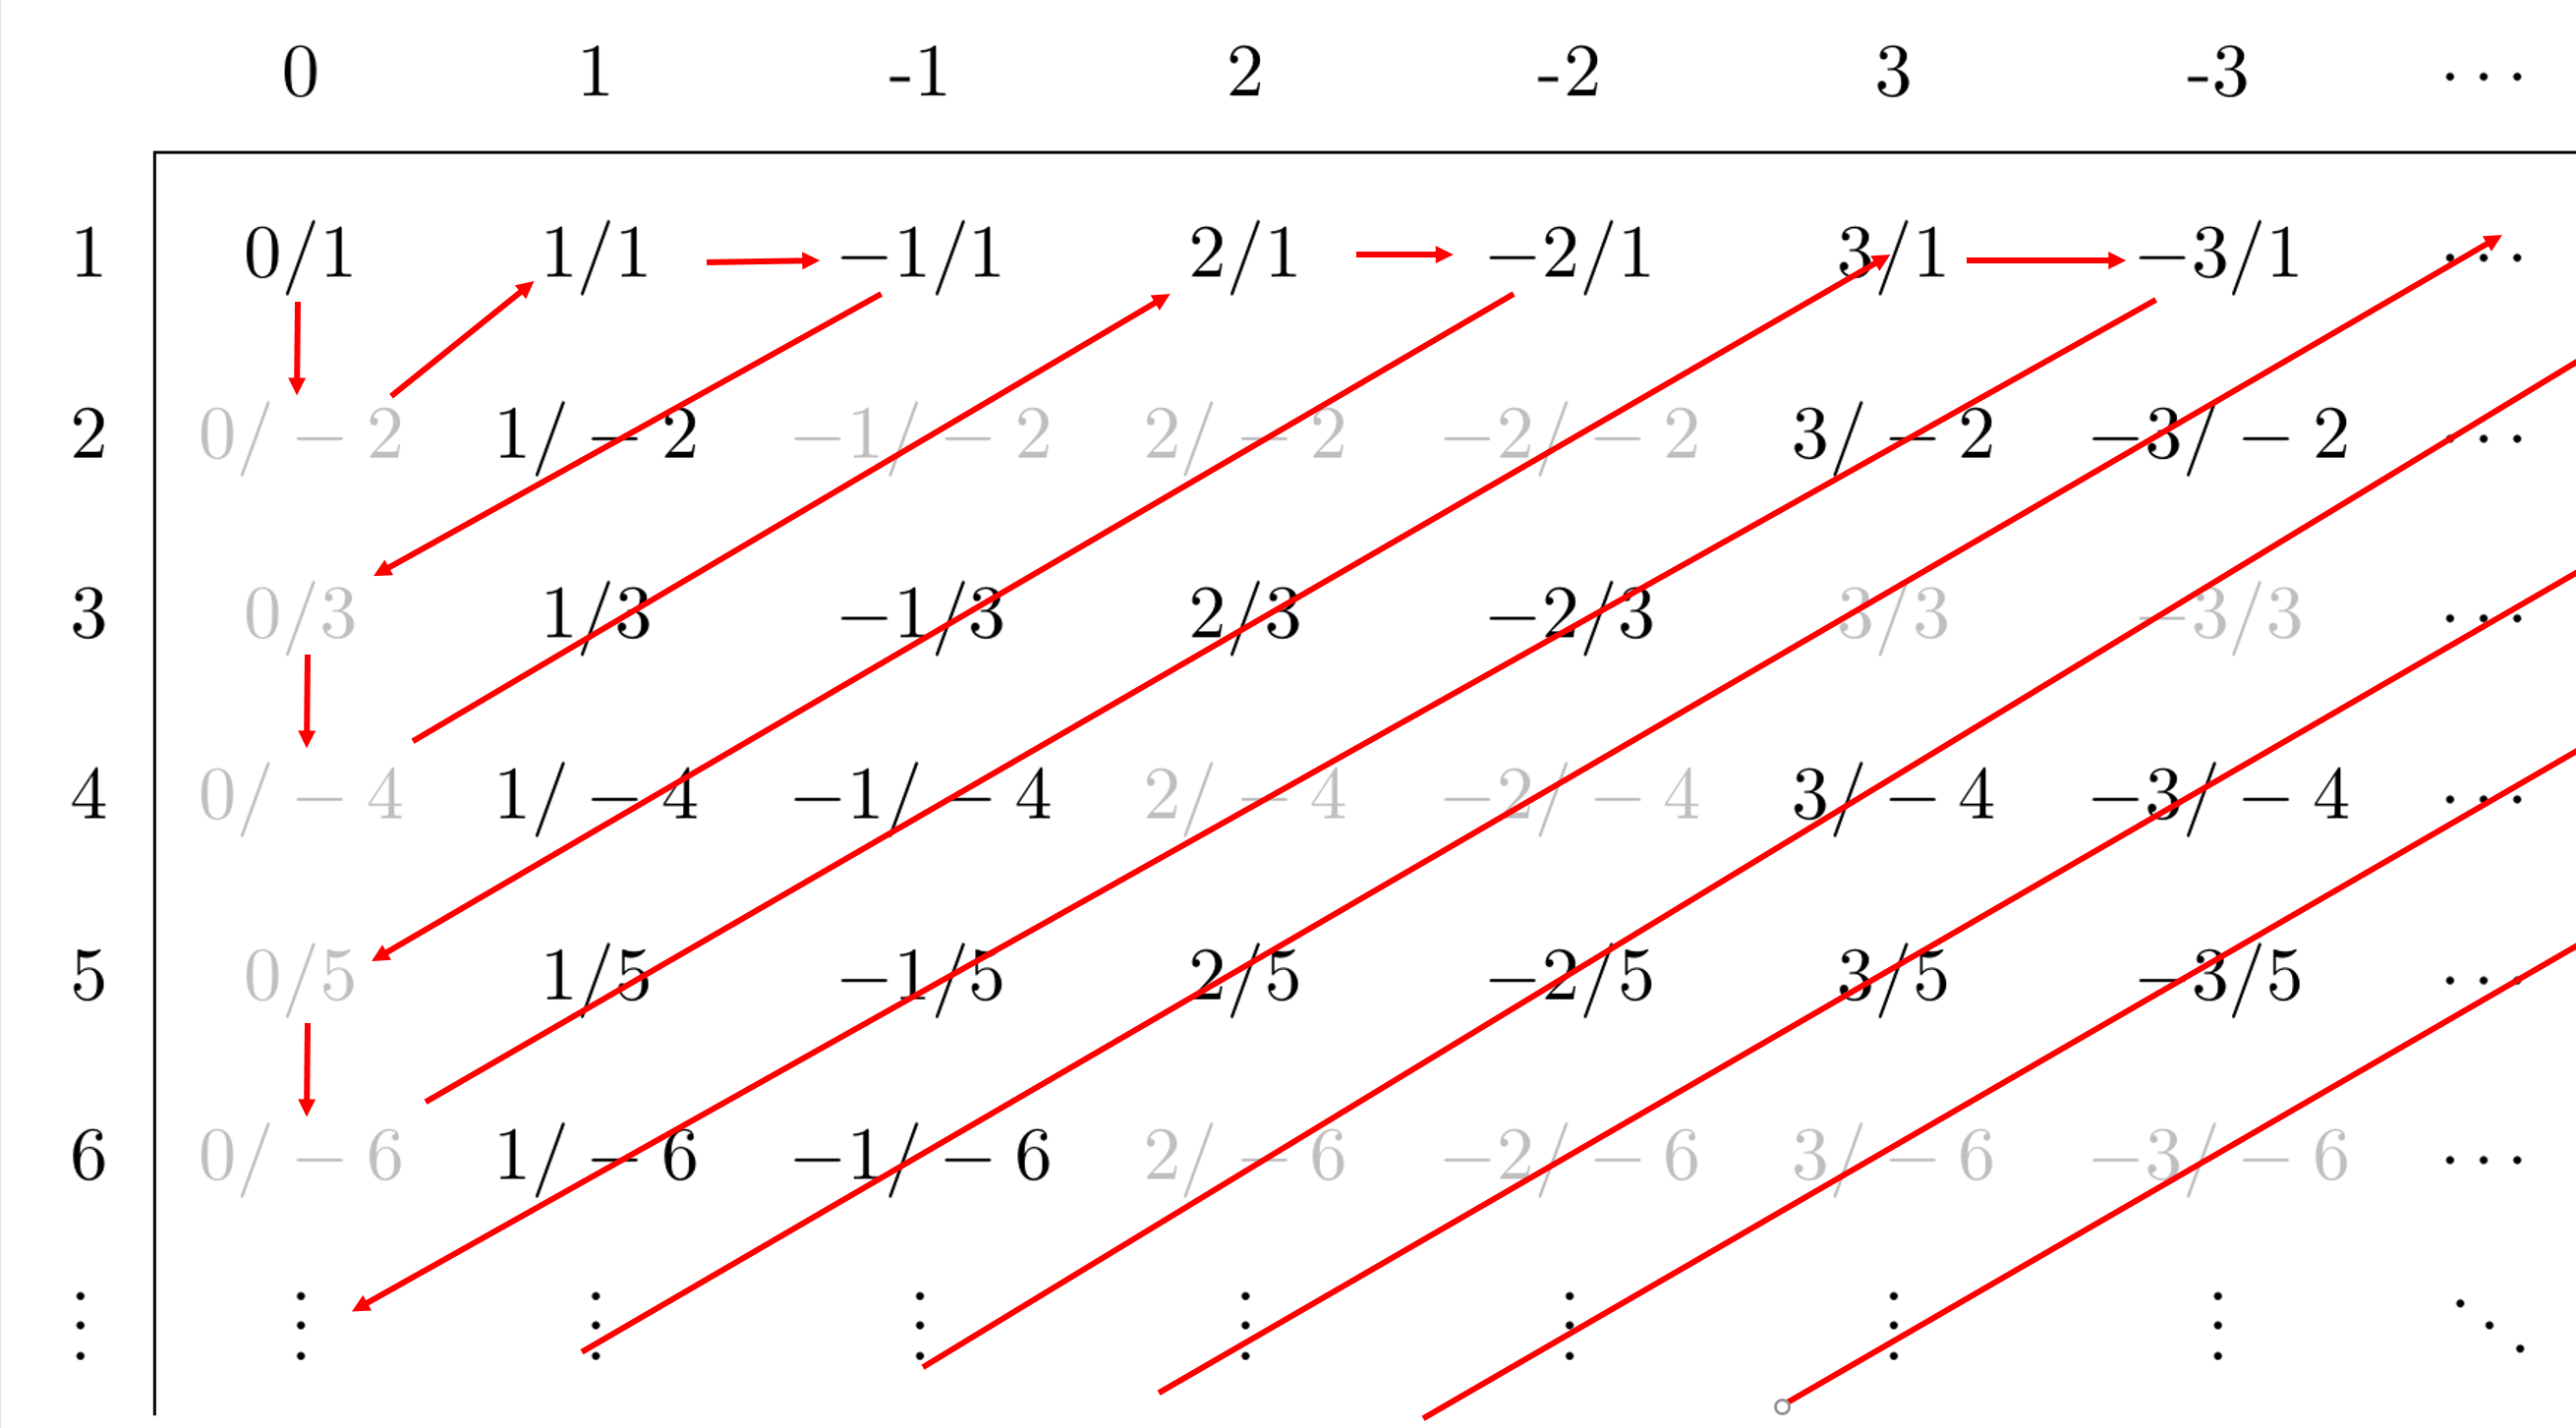
\includegraphics[width=0.7\linewidth]{figures/Qcountable}
	\caption{}
	\label{fig:qcountable}
\end{figure}


\end{proof}
\begin{proof}
	
\end{proof}
\subsection{Problems}
uniqueness of LUB

LUB property implies GLB property
\section{Point-Set Topology in Metric Spaces}
One of the main goals of calculus is to study rates of change and limiting behavior. Both of these concepts require some notion of distance, and to that end we will study \textit{metric spaces}, sets equipped with a distance function. Any such space has induced ``topological'' properties. This is a fancy way of saying that we can use distance to categorize different types of sets. Of particular interest, will be the different types of sets in $ \R $ and $ \R^n $, as the properties these sets have will have major implications down the road.  
\subsection{Metric Spaces}
Our first definition will outline how we endow a set with some notion of distance. 
\begin{definition}
	A \textit{{\color{red}metric space}} is an ordered pair $ (M,d) $ where $ M $ is a set and $ d:M\times M\to[0,\infty] $ is a function which satisfies:
	\begin{enumerate}
		\item $ d(x,y)=0 $ $ \iff $ $ x=y$.
		\item $ d(x,y)=d(y,x) $ for all $ x,y\in M $ where $ x\neq y $.
		\item $ d(x,z)\le d(x,y)+d(y,z) $ for all $ x,y,z\in M $. (Triangle Inequality)
	\end{enumerate}
\end{definition}
The function $ d $ is often called the metric, and most of its properties are compatible with our everyday understanding of distance. Firstly, distance cannot be negative. There is no distance between a point and itself. The distance from $ x $ to $ y $ is the same from $ y $ to $ x $. The final property may not be as immediate, but it is extremely important.
 
Suppose you are traveling from point $ x $ to $ z $. If you decide to take a detour to point $ y $ before heading to $ z $, then the triangle inequality ensures that you travel a weakly greater distance. An illustration shown in Figure 6 of this gives rise to the inequalities name.
\begin{figure}[h!]
	\centering
	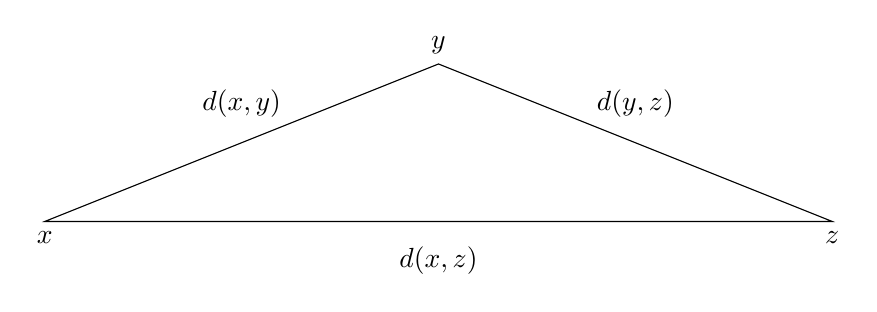
\begin{tikzpicture}
		\draw (0,0) node[anchor=north]{$x$}
		-- (10,0) node[anchor=north]{$z$}
		-- (5,2) node[anchor=south]{$y$}
		-- cycle;
		\draw (5,-0.5) node {$ d(x,z) $};
		\draw (2.5,1.5) node {$ d(x,y) $};
		\draw (7.5,1.5) node {$ d(y,z) $};
	\end{tikzpicture}
	\caption{The triangle inequality.}
\end{figure}  
Geometrically, this is equivalent to saying that the length of any side of a triangle cannot be greater than the sum of the other two lengths. Whenever presented with a weak inequality, it is often helpful to ask ``when does this hold with equality''? In this case the answer is when $ y $ is on the line segment formed by $ x $ and $ z $. In this case going to $ y $ isn't a detour at all, but just a trivial stop on the way from $ x $ to $ z $! 
\begin{example}[Euclidean Metric]
The real line $ \R $ is a metric space when equipped with the metric $ d(x,y)=|x-y| $. 
\end{example}
\begin{example}[Euclidean Metric]
Euclidean space $ \R^n $ is a metric space when equipped with the metric $$ d(\mathbf{x},\mathbf{y})=|\x-\y|=\sqrt{(x_1-y_1)^2+\cdots+(x_n-y_n)^2} .$$
\end{example}
\begin{example}[Taxi-Cab Metric]
If our set is $ \R^2 $ we can let $ d(\mathbf{x},\mathbf{y})=|x_1-y_1|+|x_2-y_2| $. This is often referred to as the taxi-cab metric, as it is how you would measure distance if driving a car on a grid. 
\end{example}
\begin{example}[$ p $-Adic Metric]
The previous examples are easy to verify, but this may not always be the case. Suppose are set is $ \Z $ and $ d:\Z\times\Z\to[0,\infty] $ is defined as $$ d(x,y)=\begin{cases}
0\text{ if }x=y\\p^{-\max\{m\in\N|\ p^m|(x-y) \}}\text{ otherwise}
\end{cases}$$ for some prime number $ p $. Before we verify this is a metric, it's worth getting a feel for how the metric actually works. If $ x\neq y $, then the distance between two points is $ p $ raised to some negative power. That negative power is defined to be the maximum whole number $ m $ such that $ (x-y) $ is divisble by $ p^m $. This gives us the vague idea that distance between points $ x $ and $ y $ is somehow related to how many times $ p $ shows up in the prime factorization of $ (x-y) $ (where $ m $ is the number of times). Let's take $ p=3 $, and pick several points in $ \Z $ to measure the distance between.    
\begin{center}
\begin{tabular}{cccccc}
	$ x $ & $ y $ & $ x-y $ & prime factorization of $ x-y $ & $ m $ & $ p^{-m} $ \\ \hline
	$ 100 $& 19  &  $ 81 $   &          $ 3^4 $                  &  $ 4 $  &     $ 1/81 $                  \\
$ 368 $	& 8  &  $ 360 $   &            $ 2^3\cdot5\cdot9 $                &  $ 0 $  &  $ 1 $                     \\
$ 35 $	& $ 5 $  &  $ 30 $   &  $ 2\cdot 3\cdot 5 $                           &      $ 1 $ & $ 1/3 $                 
\end{tabular}
\end{center}
It turns out that the more factors of $ p $ that go into the prime factorization of $ (x-y)$, the closer $ x $ and $ y $ are. Furthermore, the maximum distance between any two points is $ 1 $, as $ p^0=1 $ for all $ p $. We will now verify that this is indeed a metric. 
\begin{enumerate}
\item The function $ d(x,y) $ is defined such that $ d(x,y)=0 $ if and only if $ x=y $. 
\item We have $ (x-y)=-(y-x) $. Therefore, the prime factorization of each number differ only in sign, and give the same value $ m $. This implies that $ d(x,y)=d(y,x) $.  
\item Note that to show $ d(x,z)\le d(x,y)+d(y,z) $ for all points in $ \Z $, it suffices to show that $ d(x,z)\le\max\{d(x,y),d(y,z)\} $. This inequality happens to be a stronger condition that implies the triangle inequality. Suppose $ p^m\mid(x-y) $ and $ p^n\mid(y-z) $. For some $ s,r\in\Z $, we having
\begin{align*}
	x-y=p^mr\\y-z=p^ns.
\end{align*}
We can combine these equations to conclude $$x-z=(x-y)+(y-z)=p^mr+p^ns. $$ If $ m>n $, then $ x-z=p^n(p^{m-n}r+s)$ and $ d(x,z)=d(y,z) $. Similarly, if $ n>m $, $ d(x,z)=d(x,y) $. Finally if $ n=m $, then $$x-z=p^n(r+s)=p^m(r+s), $$ and $ d(x,z)=d(x,y)=d(y,z) $. These three cases gives the desired inequality. 
\end{enumerate}
\end{example}
The metric space we are most interested in is of course $ \R^n $ equipped with the familiar Euclidean metric. We can use this metric to define the notion of an open or closed ball in $ \R^n $. 
\begin{definition}
	If $ \x\in\R^n $ and $ r>0 $, the \textit{\color{red} open ball} with center $ \x $ and radius $ r $ is defined as $$ B_r(\x)=\{\y\in\R^n\mid|\y-\x|<r\}. $$ 
\end{definition} 
\begin{definition}
	If $ \x\in\R^n $ and $ r>0 $, the \textit{\color{red} closed ball} with center $ \x $ and radius $ r $ is defined as $$ \bar{B}_r(\x)=\{\y\in\R^n\mid|\y-\x|\le r\}. $$ 
\end{definition}
Open and closed balls in $ \R^n $ are a generalization of the open and closed intervals you were first introduced to in high school, and Figure 5 provides an illustration in $ \R^2 $. 
\begin{figure}[h!]
	\centering
	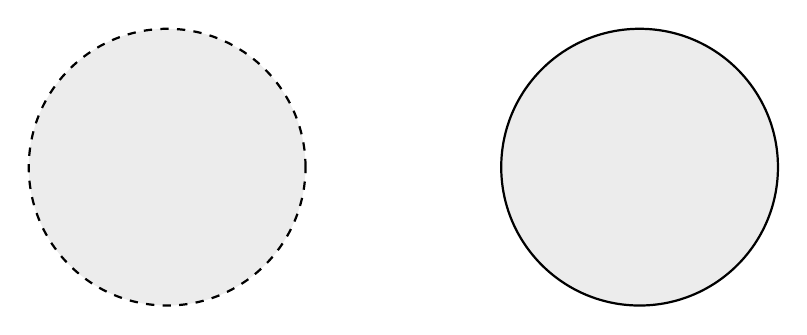
\begin{tikzpicture}
	\filldraw[color=black, fill=gray!15, thick, dashed] (0,0) circle (50pt);
	\filldraw[color=black, fill=gray!15, thick ] (6,0) circle (50pt);
	\end{tikzpicture}
	\caption{Open and closed balls in $ \R^2 $.}
\end{figure}  
\subsection{Open and Closed Sets}
We want to generalize the notion of open and closed balls in $ \R^n $ to any metric space. In order to do these, we'll need to outline a couple preliminary definitions that classify the elements of a metric space. 
\begin{definition}
	A \textit{\color{red}neighborhood } of $ x $ in a metric space $ X $ is defined as $ N_r(x)=\{y\in X\mid d(x,y)<r\} $ for a radius $ r>0 $.  
\end{definition}
As the name implies, a neighborhood centered at $ x $ is simply all the points ``around'' $ x $. Much like the open ball of Definition 3.2, neighborhoods do not include the points that are exactly a distance of $ r $ away from the point $ x $. In fact, if our metric space is $ \R^n $ with the standard metric, a neighborhood and open ball are precisely the same. 
\begin{example}
	Let our metric space be $ \Z^2 $ equipped with the taxi-cab metric. Figure 6 shows the neighborhood center at the origin of radius 3. 
		\begin{figure}[h]
		\centering
		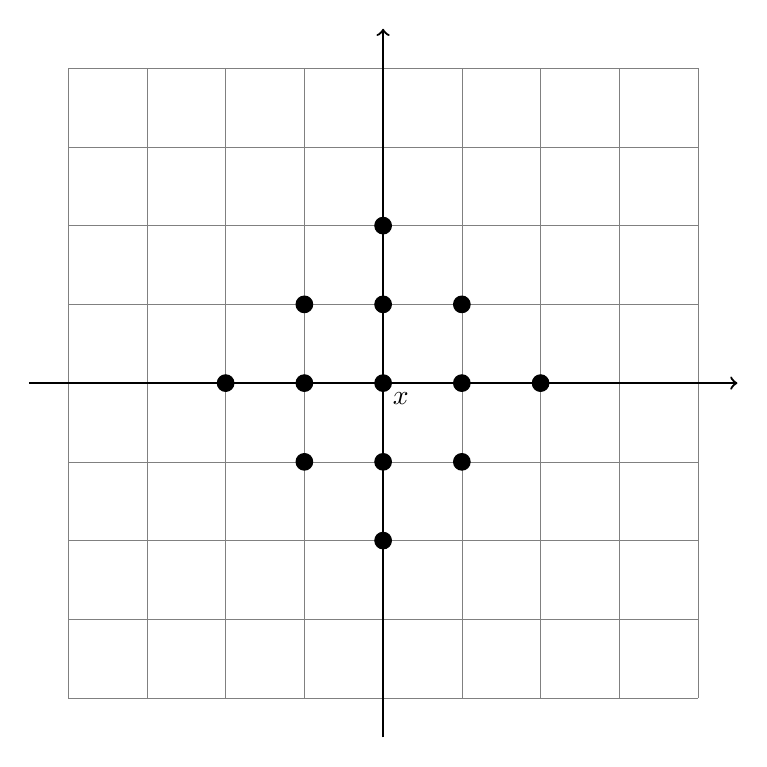
\begin{tikzpicture}
		\draw[step=1cm,gray,very thin] (-2,-2) grid (6,6);
		\draw[thick,->] (2,-2.5) -- (2,6.5);
		\draw[thick,->] (-2.5,2) -- (6.5,2);
		\filldraw (2,2) circle (3pt) node[anchor=north west] {$ x $};
		\filldraw (2,3) circle (3pt);
		\filldraw (2,4) circle (3pt);
		\filldraw (2,1) circle (3pt);
		\filldraw (2,0) circle (3pt);
		\filldraw (1,2) circle (3pt);
		\filldraw (1,3) circle (3pt);

		\filldraw (1,1) circle (3pt);
		
		\filldraw (0,2) circle (3pt);
		
		\filldraw (3,2) circle (3pt);
		\filldraw (3,3) circle (3pt);
		\filldraw (3,1) circle (3pt);
	
		\filldraw (4,2) circle (3pt);
	
	
		\end{tikzpicture}
		\caption{The set $ N_{3}(\mathbf{0})=\{\y\in\Z^2\mid|y_1|+|y_2|<3 \} $.}
	\end{figure}
\end{example} 
\begin{definition}
	Let $ X $ be a metric space. A point $ x\in X $ is a \textit{\color{red}limit point} of the set $ E\subseteq X $ if \textit{every} neighborhood of $ x $ contains a point $ y\in E $, where $ y\neq x $. We will denote the \textit{\color{red} set of all limit points} of $ E $ as $ E'=\{x\in X\mid x\text{ is a limit point of }E \} $.
\end{definition}
A limit point of a set is in some sense always ``close'' to points of the set. If $ x $ is a limit point of $ E\subseteq X $, then $ N_r(x) $ will always include points other than $ x $, no matter what we take $ r $ to be! We could make $ r $ smaller and smaller, but the set $ N_r(x) $ will never just be $ x $. In this sense, a limit point can always be ``approximated'' by elements in $ E $.  
\begin{remark}
Definition $ 3.5 $ never specifically said that a limit point of some set belongs to the set. As the next example shows, being a limit point has nothing to do with whether or not a point is included in the set in question. 	
\end{remark}
\begin{example}
$\R^2$ is a good starting place. Suppose we have a set $ E\subset \R $ that for the most part forms a rectangle. The ``border'' of the rectangle is no included in $ E $. Also note that $ E $ includes am ``isolated'' point $ z $. Let's consider three point in $ \R^2 $: $ x $, $ y $, and $ z $.  
		\begin{figure}[h]
	\centering
	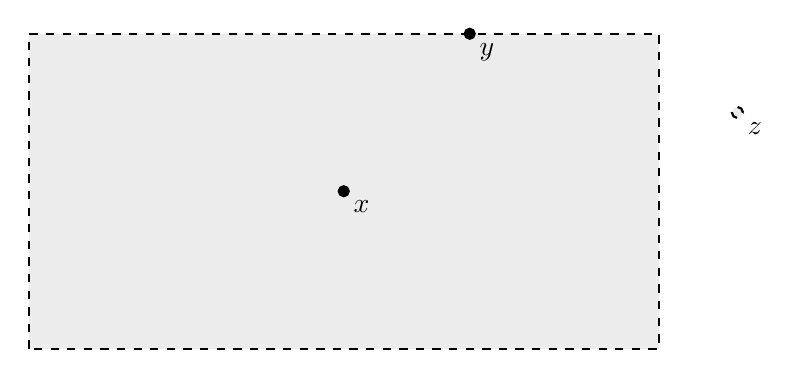
\begin{tikzpicture}
	\filldraw[color=black, fill=gray!15, thick, dashed] (0,0) rectangle (8,4);
	\filldraw (4,2) circle (2pt)node[anchor=north west] {$ x $};
	\filldraw (5.6,4) circle (2pt)node[anchor=north west] {$ y $};
	\filldraw[color=black, fill=gray!15, thick, dashed] (9,3) circle (2pt)node[anchor=north west] {$ z $};
	\end{tikzpicture}
	\caption{The set $ E\subset \R^2 $.}
\end{figure}

The point $ x $ belongs to $ E $. Furthermore, no matter what we take $ r $ to be, $ N_r(x) $ will never become a singleton of just $ \{x\} $. For the sake or argument, suppose $ x=(2,2) $. If $ r=0.5 $, then $ (2,2.49)\in N_{0.5}(x) $. Of $ r=0.01 $, then we still have $ (2,2.001)\in N_{0.01}(x) $. In fact, for every $ r $, we have $ (2,2+r/2)\in N_r(x) $. This means that $ x $ is a limit point of $ E $. 

Now consider $ y $. This point does not belong to $ E $, but it is still a limit point! We could repeat the same argument we made for $ x $ without running into trouble, because every neighborhood of $ y $ will include points ``just below'' $ y $, all of which are in $ E $! What matters with limit points is not what set the point belongs to, but what set the points nearby it belong to. 

Lastly, the point $ z $ is not a limit point. If we took $ r $ to be sufficiently large, then $ N_r(z) $ would include points in $ E $ that form the rectangle. Unfortunately, we could easily take $ r$ to be so small that $ N_r(z)=\{z\} $. It only takes one such $ r $ to rule out the chance of $ z $ being a limit point. We can provide a definition that corresponds to points like $ z $.     
\end{example}

\begin{definition}
		Let $ X $ be a metric space. For a set $ E\subseteq X $, $ x\in E $ is an \textit{\color{red}isolated point} if it is not a limit point. 
\end{definition}
By the definition of an isolated point, it is the opposite of a limit point, rendering the two definitions mutually exclusive. Every point of $ X $ must fall into the catagory of limit point or that of isolated point. For the two definitions this section is building to, this is not the case, even though it is tempting to think it is! 
\begin{definition}
Let $ X $ be a metric space. A point $ x\in X$ is an \textit{\color{red}interior point} of $ E\subseteq X $ if there exists \textit{a single} $ r>0 $ such that $ N_r(x)\subset E $. 
\end{definition}
\begin{example}
	Again, let's look at an example in $ \R^2 $. Let $ E\subset \R^2 $ be a closed ball that is ``punctured'' at $ z\in\R^2 $ such that $ z\notin E$. This can be seen in figure 8.  
\begin{figure}[h]
	\centering
	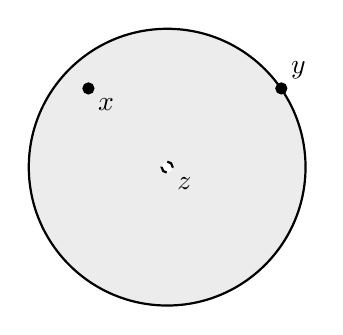
\begin{tikzpicture}
	
		\filldraw[color=black, fill=gray!15, thick ] (6,0) circle (50pt);
		\filldraw[color=black, fill=white, thick, dashed] (6,0) circle (2pt)node[anchor=north west] {$ z $};
		\filldraw (5,1) circle (2pt)node[anchor=north west] {$ x $};
		\filldraw (7.45,1) circle (2pt)node[anchor=south west] {$ y $};
	\end{tikzpicture}
	\caption{The set $ E\subset \R^2 $.}
\end{figure}	
\end{example}
\begin{remark}
	While a limit point of $ E\subset X $ need not be a point in $ E $, an interior point of $ E $ must be an element of $ E $. If $ x $ is an interior point, then $ x\in N_r(x)\subset E $ for some $ r $, so $ x\in E $. 
\end{remark}
\begin{definition}
	Let $ X $ be a metric space. A set $ E\subseteq X $ is \textit{\color{red}open} if every point of $ E $ is an interior point.  
\end{definition}
\begin{definition}
	Let $ X $ be a metric space. A set $ E\subseteq X $ is \textit{\color{red}closed} if it contains all its limit points. That is, $ E'\subseteq E $. 
\end{definition}
\begin{example}
	open and closed balls in $ \R^2 $
\end{example}
\begin{example}
	open set
\end{example}
\begin{example}
	closed set
\end{example}
\begin{remark}
	closed and open are not opposite or mutually exclusive
\end{remark}
\begin{remark}
	It's important to remember what metric space we're in!
\end{remark}
\begin{example}
	$ \Z $ in $ \Z $ vs. $ \Z $ in $ \R $. 
\end{example}
\subsection{Properties of Open and Closed Sets}
\begin{proposition}
	Every neighborhood is an open set.
\end{proposition}
\begin{proposition}
	If $ x $ is a limit point of $ E $ ($ x\in E' $), then every neighborhood of $ x $ contains infinitely many points of $ E $.
\end{proposition}
\begin{corollary}
A finite set has no limit points.
\end{corollary}
\begin{theorem}
	A set $ E $ is open \textit{if and only if} its complement is closed.
\end{theorem}
\begin{corollary}
	A set $ E $ is closed \textit{if and only if} its complement is open.
\end{corollary}
\begin{example}
	content...
\end{example}
\begin{theorem}
	Let $ \{G_\alpha\} $ and $ \{F_\alpha\} $ be an arbitrary collection of open sets and closed sets respectively. Let $ G_1,\ldots,G_n $ and $ F_1,\ldots, F_n $ be a finite collection of open sets and closed sets respectively. In this case we have:
	\begin{enumerate}
		\item $ \bigcup_\alpha G_\alpha $ is open.
		\item $ \bigcap_\alpha F_\alpha $ is closed.
		\item $ \bigcup_{i=1}^n G_i$ is open.
		\item $ \bigcap_{i=1}^n F_i$ is closed.
	\end{enumerate}
\end{theorem}
\begin{example}

\end{example}
\subsection{Closures, Interiors, Dense Sets, and Perfect Sets} 
\begin{definition}
Let $ X $ be a metric space. The \textit{\color{red}interior} of a set $ E\subset X $, denoted $ E^\circ $, is the set of all interior points of $ E $. 
\end{definition}
\begin{definition}
	Let $ X $ be a metric space. The \textit{\color{red}closure} of a set $ E\subset X $ is $ \bar{E}=E\cup E' $. 
\end{definition}
\begin{definition}
	Let $ X $ be a metric space. The set $ E\subset X $ is \textit{\color{red}perfect} if every point of $ E $ is a limit point of $ E $. 
\end{definition}
\begin{definition}
	Let $ X $ be a metric space. The set $ E\subset X $ is \textit{\color{red}dense in $ X $} if every point of $ X $ is a limit point of $ E $, or a point of $ E $. ($ \bar{E}=X $)  
\end{definition}
\subsection{Compact Sets}
\subsection{Properties of Compact Sets}

\section{Sequences and Series}
\subsection{Convergence}
density
\subsection{Subsequences}
\subsection{Cauchy Sequences}
\subsection{Extending $ \R $}
\subsection{$ \limsup $ and $ \liminf $}
\subsection{Series}

\section{Continuity}
\subsection{Limits of Functions}
\subsection{Continuous Functions}
\subsection{Intermediate Value Theorem}
\subsection{Uniform Continuity}
\subsection{Continuity and Compactness}
\subsection{Discontinuities}
\subsection{Monotonicity}
\section{Differentiation}
\subsection{The Definition of a Derivative}
\subsection{Properties of the Derivative}
\subsection{The Chain Rule}
\subsection{Mean Value Theorem}
\subsection{L'H\^{o}pital's Rule}
\section{Riemann Integration}
\subsection{Partitions}
\subsection{Simple Functions}
\subsection{Upper and lower Riemann Integrals}
\subsection{Properties of the Riemann Integral}
\subsection{Integration with Continuity and/or Monotonicity}
\subsection{Riemann-Stieltjes Integral}
\section{Sequences and Series of Functions}
\subsection{Sequences}
\subsection{Convergence}
\subsection{Uniform Convergence}
\subsection{Properties of Uniform Convergence}
\subsection{Series}
\subsection{Power Series}
\subsection{Taylor Series}
\section{Functions of Several Variables}
\subsection{Linear Transformations}
\section{Differentiation with Several Variables}
\subsection{The Derivative as a Linear Map}
\subsection{The Chain Rule}
\subsection{The Inverse Function Theorem}
\subsection{The Implicit Function Theorem}
\section{Riemann Integration with Several Variables}
\subsection{Integration over a Rectangle}
\subsection{Iterated Integrals}
\subsection{Change of Variables}
\subsection{Change of Variables, Proof}
\section{Differential Forms}
\subsection{Motivation and Review of Vector Calculus}
\subsection{Tensors}
\subsection{Wedge Product}
\subsection{Tangent Vectors and Differential Forms}
\subsection{Manifolds}
\subsection{Stokes' Theorem}
\section{Measures}
\subsection{Motivation}
\subsection{$ \sigma $-Algebras}
\subsection{Measures}
\subsection{Outer Measures}
\subsection{Measures on $ \R $}
\section{Integration Revisited}
\subsection{Measurable Functions}
\subsection{Itegration of Simple Functions}
\subsection{Integration of Nonnegative Functions}
\subsection{Integration of Real Functions}
\subsection{Product Measures}
\subsection{Lebesgue Integration in $ n- $Dimensions}
\section{Differentiation with Measures}
\subsection{Motivation in $ \R $}
\subsection{Signed Measures}
\subsection{Radon-Nikodym Derivative}
\section{Foundations of Functional Analysis}
\subsection{Normed Vector Spaces}
\subsection{Linear Functionals}
\subsection{The Baire Category Theorem}
\subsection{Hilbert Spaces}
\section{$ L^p $ Spaces}
\subsection{Basic Theory}
\subsection{The Dual of $ L^p $}
\subsection{Inequalities}
\section{Radon Measures}
\section{Foundations of Fourier Analysis}
\section{Convex Analysis}
\newpage
\bibliography{analysis}{} 
\end{document}